%\section{Title @Venue'Year}
%\subsection{Background/Problems}
%\subsection{Methods/Techniques}
%\subsection{Results/Evaluation}
%\subsection{Limitations/Comments}
%\newpage
%\begin{figure}[h]
%    \centering
%    \includegraphics[width=\linewidth]{xx.png} %
%    \caption{xx's arch.}	
%    \label{fig:xx}
%\end{figure}
\documentclass[10pt]{article} %twocolumn
%\usepackage{ctex}
\usepackage{titlesec}
\usepackage{titletoc}
\titleformat*{\section}{\normalfont\bfseries} %\tiny\scriptsize\footnotesize\small\normalsize\large\Large\LARGE\huge\Huge
\titleformat*{\subsection}{\normalfont\bfseries}
\usepackage{graphicx}
\usepackage{url}
\usepackage{listings}
\usepackage[colorlinks,linkcolor=black,anchorcolor=blue,citecolor=green]{hyperref}%
%for pdftex
%\setlength{\pdfpageheight}{160mm}
%\setlength{\pdfpagewidth}{80mm}

%for dvipdfm
%\special{pdf: pagesize width 80mm height 160mm}

%\setcounter{secnumdepth}{3}		%编号深度
\setcounter{tocdepth}{1}		%目录深度
\titlecontents{section}[0mm]%标签距离页面左边距
{\footnotesize}
%{\fontsize{10pt}{10pt}} %\selectfont
{\contentslabel{1em}}  %标签距离目录内容距离
{}
{\titlerule*{.}\contentspage}[\addvspace{.5pc}]


\let\phone=1 %-------------生成适合手机上阅读的pdf文件;否则注释此行。------------------
\ifx\phone1
\usepackage[centering,margin=0.5cm]{geometry}
\geometry{papersize={12cm,20cm}} 
\else
\usepackage[a4paper,margin=2cm]{geometry}%,left=2cm,right=2cm,top=1cm,bottom=1cm
\twocolumn
\fi


%for dvips
%\special{papersize=80mm,160mm} %dvi 没有纸张大小的概念,只有转换成 .ps、.pdf 文件时,才由对应的输出驱动(如 Dvips、dvipdfmx 或 pdfTeX 等)设置输出纸张大小。
%传统的 TeX 代码里面本身不能直接设置纸大小,因此才需要在安装 TeX Live 时选择那些输出驱动的默认纸张大小。而 article 等文档类的 a4paper、letterpaper 选项,只是设置合适的版心位置和距离,以适合这些纸张大小。
%不过,在 TeX 代码里面用特定输出驱动的 special 命令,可以提示这些输出驱动选择纸张,一般用 geometry 宏包的话,就会处理这个问题。而 graphics 宏包后台对 pdfTeX 也有相应的代码(在 pdftex.def 中)。


\title{\textbf{Reading Notes}}%文献阅读笔记
\author{\texttt{TSISers} 
    \\ \copyright Trusted Software and Intelligent System Lab.}
\date{2020/01/21}

\begin{document}

\maketitle 
\tableofcontents
\clearpage



\section{SAVIOR: Towards Bug-Driven Hybrid Testing @S\&P'20
}

\subsection{Background/Problems}
Hybrid testing combines fuzzing and concolic
execution. It leverages fuzzing to test easy-to-reach code
regions and uses concolic execution to explore code blocks
guarded by complex branch conditions. As a result, hybrid testing
is able to reach deeper into program state space than fuzz
testing or concolic execution alone. Recently, hybrid testing has
seen significant advancement. However, {its code coverage-centric
design is inefficient in vulnerability detection}. First, it {blindly}
selects seeds for concolic execution and aims to explore new code
continuously. However, as statistics show, a large portion of the
explored code is often bug-free. Therefore, giving equal attention
to every part of the code during hybrid testing is a non-optimal
strategy. It slows down the detection of real vulnerabilities by
over 43\%. Second, classic hybrid testing quickly moves on after
reaching a chunk of code, rather than examining the hidden
defects inside. It may frequently {miss subtle vulnerabilities}
despite that it has already explored the vulnerable code paths.
\subsection{Methods/Techniques}
The authors propose SAVIOR (Fig.\ref{fig:savior}), a new hybrid testing framework pioneering
a bug-driven principle.

\textbf{Bug-driven prioritization:} Instead of running all seeds without
distinction in concolic execution, SAVIOR prioritizes
those that have higher possibilities of leading to vulnerabilities.
Specifically, before the testing, SAVIOR analyzes the source
code and {statically labels the potentially vulnerable locations}
in the target program.
Moreover, SAVIOR computes the set of basic blocks reachable
from each branch. During dynamic testing, SAVIOR {prioritizes the concolic execution seeds that can visit more
important branches} (i.e., branches whose reachable code has
more vulnerability labels).  

\textbf{Bug-guided verification: }Aside from accelerating vulnerability
detection, SAVIOR also verifies the labeled vulnerabilities
along the program path traversed by the concolic executor.
Specifically, SAVIOR synthesizes the faulty constraint of
triggering each vulnerability on the execution path. If such
constraint under the current path condition is satisfiable,
SAVIOR solves the constraint to construct a test input as
the proof. Otherwise, SAVIOR proves that the vulnerability
is infeasible on this path, regardless of the input.

\begin{figure}[h]
    \centering
    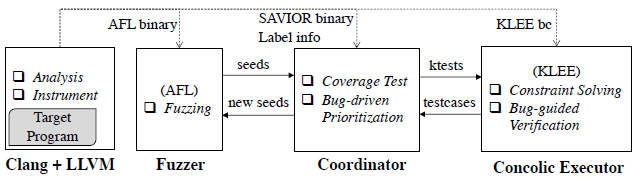
\includegraphics[width=\linewidth]{savior.png} %
    \caption{SAVIOR's arch.}	
    \label{fig:savior}
\end{figure}


\subsection{Results/Evaluation %评估效果
}
Evaluation shows that the bug-driven approach outperforms mainstream
 hybrid testing systems driven by code coverage. On average, SAVIOR
detects vulnerabilities 43.4\% faster than DRILLER and 44.3\%
faster than QSYM, leading to the discovery of 88 and 76 more
unique bugs, respectively. According to the {evaluation on 11 well
fuzzed benchmark programs, within the first 24 hours, SAVIOR
triggers 481 UBSAN violations, among which 243 are real bugs.}

\subsection{Limitations/Comments}
\begin{itemize}
    \item Over-approximation in Vulnerability Labeling: SAVIOR leverages sound algorithms
to label vulnerabilities where the over-approximation may
introduce many false-positive labels. This imprecision can
consequently weaken the performance of SAVIOR's prioritization. 
One solution is to include more precise
static analysis for finer-grained label pruning.
    \item Prediction in Vulnerability Detection: Once reaching a
potentially vulnerable location in concolic execution,
SAVIOR extracts the guarding predicates of the vulnerability
label. However, these predicates may contradict the current
path condition. In case of such contradiction, SAVIOR terminates
the exploration of the labeling site immediately.
Moreover, we can predict whether an execution
path can trigger a vulnerability or not by studying the
runtime information of previous executions, more importantly,
before that execution arrives the vulnerability site. To
achieve this goal, we need to backwardly summarize
path constraints from the labeled site to its predecessors in
the explored paths, by using the weakest precondition.
    \item Hybrid testing in SAVIOR is same with hybrid fuzzing in Driller and Berry. Both tools run fuzzing for code exploration and invoke concolic execution only on
hard-to-solve branches, which takes advantage of both fuzzer's
efficiency and concolic executor's constraint solving.
\end{itemize}
\newpage
\section{Fuzzing File Systems via Two-Dimensional Input Space Exploration @S\&P'19}
\subsection{Background/Problems}
File systems are too big and too complex to be bug free. Nevertheless, to find bugs in file systems, regular stress-testing tools and formal checkers are limited due to the ever-increasing complexity of both file systems and OSes. Thus, fuzzing becomes a preferable choice, as it does not need much knowledge about a target. However,
three prominent issues of existing file systems fuzzers exist: 
(1) fuzzing a large blob image is inefficient; 
(2) fuzzers do not exploit the dependence
between a file system image and file operations; 
(3) fuzzers use aging OSes and file systems, which results in
irreproducible bugs.

\subsection{Methods/Techniques}
The authors present JANUS (Fig.\ref{fig:janus}, 120K C++/C LoC), the first feedback-driven fuzzer
that explores the two-dimensional input space of a file system,
i.e., mutating metadata on a large image, while emitting image-directed
file operations. In addition, JANUS relies on a library
OS rather than on traditional VMs for fuzzing, which enables
JANUS to load a fresh copy of the OS, thereby leading to better
reproducibility of bugs.
\begin{figure}[h]
    \centering
    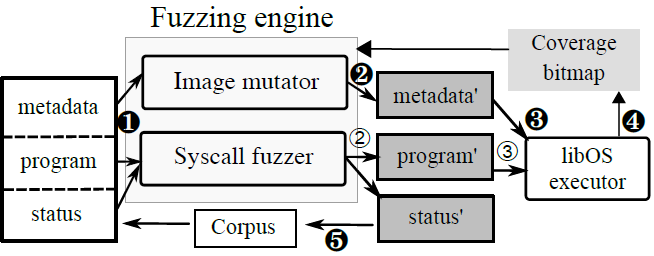
\includegraphics[scale=0.5]{janus.png} %
    \caption{JANUS' arch.}	
    \label{fig:janus}
\end{figure}
\subsection{Results/Evaluation}
The authors evaluate JANUS on 8 file systems
and found 90 bugs in the upstream Linux kernel, 62 of which have
been acknowledged. 43 bugs have been fixed with 32
CVEs assigned. In addition, JANUS achieves higher code coverage
on all the file systems after fuzzing 12 hours, when compared
with the state-of-the-art fuzzer Syzkaller.
JANUS visits 4.19X and 2.01X more code paths in Btrfs and ext4,
respectively. Moreover, JANUS is able to reproduce 88–100\% of
the crashes, while Syzkaller fails on all of them.
\subsection{Limitations/Comments}
\begin{itemize}
    \item JANUS cannot fuzz the DAX mode of a file system without modification on LKL. 
    \item To achieve a minimal PoC, JANUS uses a brute force approach to revert
every mutated byte and also tries to remove every invoked
file operation to check whether the kernel still crashes at the
expected location, which is sub-optimal.
    \item JANUS does not support file systems (e.g., NTFS, GVfs, SSHF, etc.)
that rely on FUSE (Filesystem in Userspace).
    \item By combining Janus and kAFL, we can fuzz file systems on other OSes.
    \item Other crash-consistency checkers [6,73] and semantic correctness checkers [36, 58] can rely on or integrate with Janus which aims to find general security bugs in file systems.
    \item To find security bugs in OSes, a number
    of general kernel fuzzing frameworks [20, 43, 46, 61] and
    OS-specific kernel fuzzers [22, 25, 44, 45, 47] have been
    proposed. Unlike JANUS, all these fuzzers generate random
    system calls based upon predefined grammar rules, which is
    ineffective in the context of file system fuzzing. Several recent
    OS fuzzers such as IMF [22] and MoonShine [49] focusing
    on seed distillation are orthogonal to this work. Nevertheless,
    JANUS can start with seed programs of high quality by utilizing
    their approaches.
\end{itemize}
\newpage

\section{REDQUEEN: Fuzzing with Input-to-State Correspondence @NDSS'19}
\subsection{Background/Problems}
Two common problems of fuzzing are magic numbers
and (nested) checksums (see Listing \ref{fuzzissues}). Computationally expensive methods such
as taint tracking and symbolic execution are typically used to
overcome such roadblocks. Unfortunately, such methods often
require access to source code, a rather precise description of the
environment (e.g., behavior of library calls or the underlying OS),
or the exact semantics of the platform's instruction set, and thus 
such methods are the polar opposite of the approach pioneered by AFL: to a
large extend, AFL's success is based on the fact that it makes
few assumptions about the program's behavior.
\begin{lstlisting}[label=fuzzissues,language={[ANSI]C}, caption={Roadblocks for feedback-driven fuzzing.}]
/* magic number example */
if(u64(input)==u64("MAGICHDR"))
  bug(1);
/* nested checksum example */
if(u64(input)==sum(input+8, len-8))
  if(u64(input+8)==sum(input+16, len-16))
    if(input[16]=='R' && input[17]=='Q')
      bug(2);
\end{lstlisting}

\subsection{Methods/Techniques}
The authors introduce a lightweight, yet very effective
approach to facilitate
and optimize state-of-the-art feedback fuzzing that easily scales
to large binary applications and unknown environments. We
observe that during the execution of a given program, parts
of the input often end up directly (i.e., nearly unmodified)
in the program state. This \emph{input-to-state correspondence} can
be exploited to create a robust method to overcome common
fuzzing roadblocks in a highly effective and efficient manner.
Their prototype implementation, called REDQUEEN, is able to
solve magic bytes and (nested) checksum tests automatically
for a given binary executable. Additionally, The authors show that the
techniques outperform various state-of-the-art tools on a wide
variety of targets across different privilege levels (kernel-space
and userland) with no platform-specific code.
\subsection{Results/Evaluation}
REDQUEEN is the
first method to find more than 100\% of the bugs planted in
LAVA-M across all targets. Furthermore, The authors discovered
65 new bugs and obtained 16 CVEs in multiple programs and
OS kernel drivers. Finally, their evaluation demonstrates that
REDQUEEN is fast, widely applicable and outperforms concurrent
approaches by up to three orders of magnitude. Available at: \url{https://github.com/RUB-SysSec/redqueen}
\subsection{Limitations/Comments}
\begin{itemize}
    \item REDQUEEN cannot deal with those cases in which the input does not correspond to the state, such as compression or hash maps in the input.
    \item It would be beneficial to use this
lightweight approach as a first step where possible, and than
solve the remaining challenges using complex approaches.
\end{itemize}

\subsection*{Core design of AFL}
\hspace{2mm}{
Fuzzers from the AFL family have three important components:
(i) the queue, (ii) the bitmap, and (iii) the mutators. The queue
is where all inputs are stored. During the fuzzing process,
an input is picked from the queue, fuzzed for a while, and,
eventually, returned to the queue. After picking one input, the
mutators perform a series of mutations. After each step, the
mutated input is executed. The target is instrumented such that
the coverage produced by the input is written into a bitmap. If
the input triggered new coverage (and, therefore, a new bit
is set in the bitmap), the input is appended to the queue.
Otherwise, the mutated input is discarded. The mutators are
organized in different stages. The first stages are called the
\emph{deterministic stages}. These stages are applied once, no matter
how often the input is picked from the queue. They consist
of a variety of simple mutations such as “try flipping each
bit”. When the deterministic stages are finished or an input
is picked for the second time, the so called \emph{havoc phase} is
executed. During this phase, multiple random mutations are
applied at the same time at random locations. Similarly, if the
user provided a dictionary with interesting strings, they are
added in random positions. Linked to the havoc stage is the
\emph{splicing stage}, in which two different inputs are combined at
a random position.}
\newpage

\section{GRIMOIRE: Synthesizing Structure while Fuzzing @Security'19 }
\subsection{Background/Problems}
One common challenge for current fuzzing techniques are programs which process highly structured input languages such as interpreters, compilers, text-based network protocols or markup languages. Typically, such inputs are consumed by the program in two stages: parsing and semantic analysis. If parsing of the input fails, deeper parts of the target program—containing the actual application logic—fail to execute; hence, bugs hidden “deep” in the code cannot be reached. Even advanced feedback fuzzers— such as AFL—are typically unable to produce diverse sets of syntactically valid inputs.

Previous approaches to address this problem are typically based on manually provided grammars or seed corpora. On the downside, such methods require human experts to (often manually) specify the grammar or suitable seed corpora, which becomes next to impossible for applications with undocumented or proprietary input specifications. An orthogonal line of work tries to utilize advanced program analysis techniques to automatically infer grammars. Typically performed as a pre-processing step, such methods are used for generating a grammar that guides the fuzzing process. However, since this grammar is treated as immutable, no additional learning takes place during the actual fuzzing run.

\subsection{Methods/Techniques}
The authors present the design and implementation of GRIMOIRE, a fully automated coverage-guided fuzzer which works without any form of human interaction or pre-configuration; yet, it is still able to efficiently test programs that expect highly structured inputs. Thet achieve this by performing large-scale mutations in the program input space using grammar-like combinations to synthesize new highly structured inputs without any pre-processing step. 

 Their approach is based on two key observations: First, they can use code coverage feedback to automatically infer structural properties of the input language. Second, the precise and “correct” grammars generated by previous approaches are actually unnecessary in practice: since fuzzers have the virtue of high test case throughput, they can deal with a significant amount of noise and imprecision. In fact, in some programs (such as Boolector) with a rather diverse set of input languages, the additional noise even benefits the fuzz testing. In a similar vein, there are often program paths which can only be accessed by inputs outside of the formal specifications, e. g., due to incomplete or imprecise implementations or error handling code.
\begin{figure}[h]
    \centering
    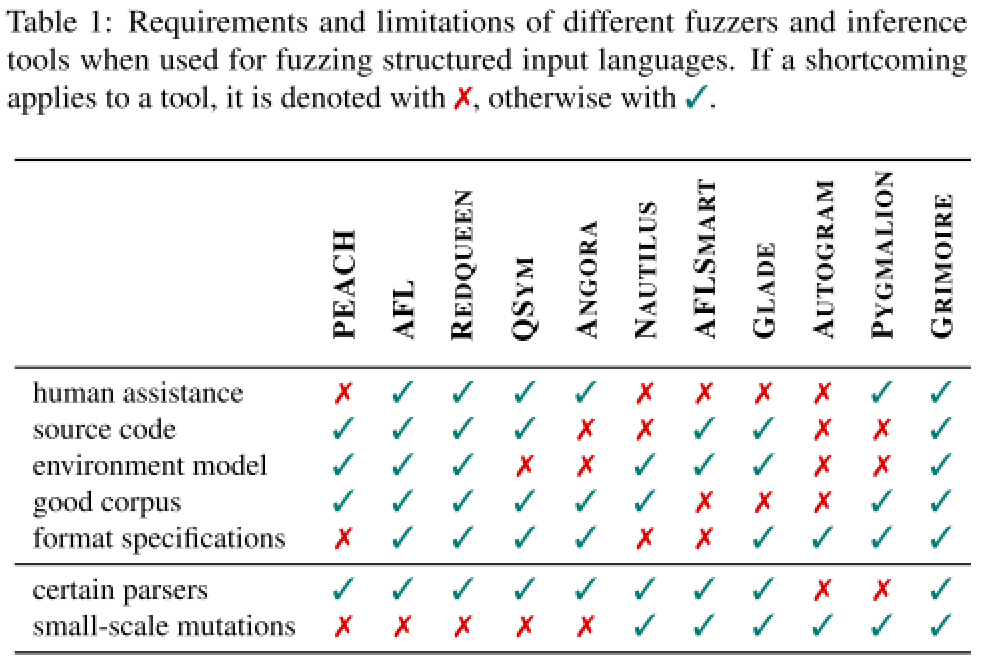
\includegraphics[width=\linewidth]{grimoire.png} %
    \caption{Advantage of Grimoire.}	
    \label{fig:janus}
\end{figure}
\subsection{Results/Evaluation}
 First, The authors evaluate GRIMOIRE against other fuzzers on four scripting language interpreters (mruby, PHP, Lua and JavaScriptCore), a compiler (TCC), an assembler (NASM), a database (SQLite), a parser (libxml) and an SMT solver (Boolector).  GRIMOIRE outperforms all existing coverage-guided fuzzers; in the case of Boolector, GRIMOIRE finds up to 87\% more coverage than the baseline (REDQUEEN). 

 Second, they evaluate GRIMOIRE against state-of-the-art grammar-based fuzzers. they observe that in situations where an input specification is available, it is advisable to use GRIMOIRE in addition to a grammar fuzzer to further increase the test coverage found by grammar fuzzers.
 
 Third, they evaluate GRIMOIRE against current state-of-the-art approaches that use automatically inferred grammars for fuzzing and found that they can significantly outperform such approaches. Overall, GRIMOIRE found 19 distinct memory corruption bugs that they manually verified. they responsibly disclosed all of them to the vendors and obtained 11 CVEs. During their evaluation, the next best fuzzer only found 5 of these bugs. In fact, GRIMOIRE found more bugs than all five other fuzzers combined.
 
 Available at: \url{https://github.com/RUB-SysSec/grimoire}
\subsection{Limitations/Comments}
The approach has significant difficulties with more syntactically complex constructs, such as matching the ID of opening and closing tags in XML or identifying variable constructs in scripting languages. 

The generalization approach might be too coarse in many places. Obtaining more precise rules would help uncovering deeper parts of the target application in cases where multiple valid statements have to be produced. 
\newpage
\section{Intriguer: Field-Level Constraint Solving for Hybrid Fuzzing @CCS'19}
\subsection{Background/Problems}
Hybrid fuzzing is promising in light of the recent performance improvements in concolic engines. However, there is room for further improvement: symbolic emulation is still slow, unnecessary constraints dominate solving time, resources are overly allocated, and hard-to-trigger bugs are missed.

\subsection{Methods/Techniques}
The authors present a new hybrid fuzzer named Intriguer (Fig.\ref{fig:intriguer}). The key idea of Intriguer is field-level constraint solving, which optimizes symbolic execution with field-level knowledge. Intriguer performs instruction-level taint analysis and records execution traces without data transfer instructions like mov. Intriguer then reduces the execution traces for tainted instructions that accessed a wide range of input bytes, and infers input fields to build field transition trees. With these optimizations, Intriguer can efficiently perform symbolic emulation for more relevant instructions and invoke a solver for complicated constraints only.

\begin{figure}[h]
    \centering
    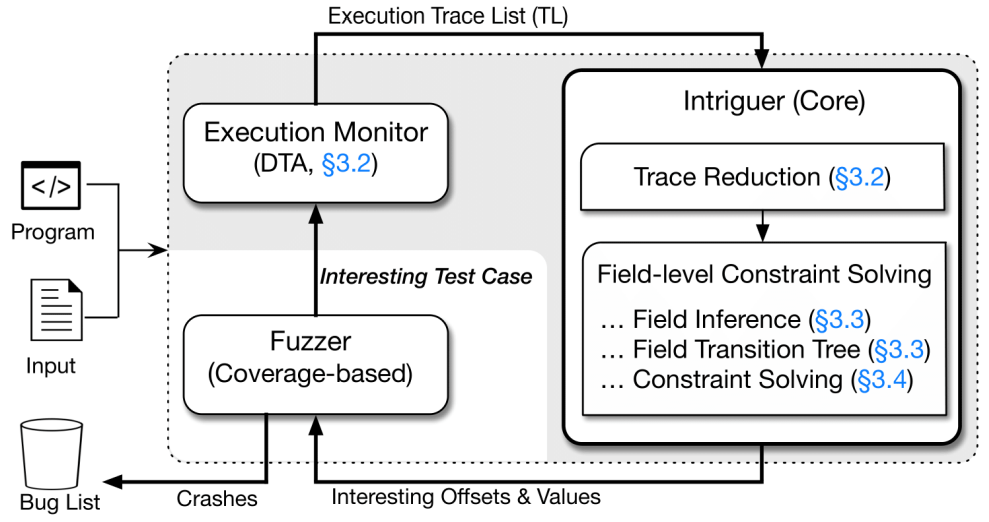
\includegraphics[width=\linewidth]{intriguer.png} %
    \caption{Intriguer's arch.}	
    \label{fig:intriguer}
\end{figure}
\subsection{Results/Evaluation}
Evaluation results indicate that Intriguer outperforms the state-of-the-art fuzzers: Intriguer found all the bugs in the LAVA-M(5h) benchmark dataset for ground truth performance, and also discovered 43 new security bugs in seven real-world programs. They reported the bugs and received 23 new CVEs.

\subsection{Limitations/Comments}
 Intriguer performed field inference by inspecting off sets recorded in the execution traces and did not consider the association between those fields.  To perform field-level constraint solving more efficiently, Intriguer should identify fields of the same type through the FL and grouping them together. In addition to identifying repeated fields, we may infer structure from those fields and then consider mutation strategies specific to repeated fields based on it.

Intriguer reduces the execution traces to emulate only the small portion of the instructions that are repeatedly used to access a wide range of input bytes. One may have two concerns regarding trace reduction. First, excessively reduced traces may affect a constraint solving for important branches. By considering the context-sensitivity of the run-time process, Intriguer will not perform trace reduction when a program is in a different context (e.g., different call stack). Second, the instructions can be repeatedly used to access only a narrow range of input bytes. Note that an execution bottleneck can also occur if the instructions are used to repetitively access the input with specific offsets. We can address this problem by reducing the execution traces for the instructions that use the same offset by considering the program’s context.

Intriguer currently supports most of the x86 instruction set and a part of x86\_64 instruction set. Although it is challenging to support all of x86\_64 instructions, we can implement frequently used instructions to support actual program execution.

The current version of Intriguer does not consider the control-flow dependency, e.g., occurring from indirect
and conditional jump.
\newpage

\section{FIRM-AFL: High-Throughput Greybox Fuzzing of IoT Firmware via Augmented Process Emulation @Sec'19}
\subsection{Background/Problems}
Two fundamental problems in \emph{IoT fuzzing} due to its strong dependency on the actual hardware configuration: 1) Compatibility issues by enabling fuzzing for POSIX-compatible firmware that can be emulated in a system emulator. 2) Performance bottleneck caused by system-mode emulation. 
\subsection{Methods/Techniques}
A novel technique called augmented process emulation. By combining system-mode emulation  (high generality and low efficiency)  and user-mode emulation  (low generality and high efficiency) in a novel way, augmented process emulation provides high compatibility as system-mode emulation and high throughput as user-mode emulation.  The program to be fuzzed is mainly run in user-mode emulation to achieve high efficiency, and switches to full system emulation only when necessary to ensure correct program execution. 
\begin{figure}[h]
    \centering
    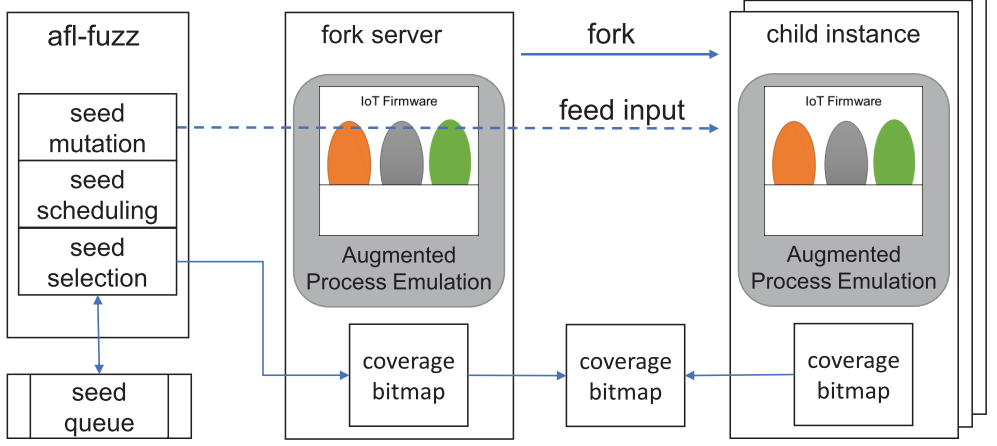
\includegraphics[width=\linewidth]{firm-afl.png} %width=\linewidth
    \caption{firm-afl's arch.}	
    \label{fig:firmafl}
\end{figure}
\subsection{Results/Evaluation}
Evaluation results show that (1) FIRM-AFL is fully functional and capable of finding real-world vulnerabilities in IoT programs; (2) the throughput of FIRM-AFL is on average 8.2 times higher than system-mode emulation based fuzzing; and (3) FIRM-AFL can find 1-day vulnerabilities much faster than system-mode emulation based fuzzing, and find 0-day vulnerabilities.

available at \url{https://github.com/zyw-200/FirmAFL}.

\subsection{Limitations/Comments}
FIRM-AFL only supports the following CPU architectures: mipsel, mipseb and armel.  It can also only fuzz a program in a firmware image that can be properly emulated by Firmadyne and runs a POSIX-compatible OS (e.g., Linux).
\clearpage

\section{RVFUZZER: Finding Input Validation Bugs in Robotic Vehicles Through
Control-Guided Testing @Security'19}
\subsection{Background/Problems}
Attack surface of robotic vehicles (RVs) spans multiple aspects, such as (1) physical vulnerabilities of its sensors that enable external sensor spoofing attacks [72,77,80]; (2) traditional “syntactic” bugs in its control program (e.g., memory corruption bugs) that enable remote or trojaned exploits [75]; and (3) control-semantic bugs in its control program that enable attacks via remote control commands.  For attacks exploiting (1) and (2), there have been research efforts in defending against them [30,38,40,50,52,70,76]; whereas those exploiting (3) have not received sufficient attention. 

 In this paper, the authors address a new type of vulnerability in RV control programs, called input validation bugs, which involve missing or incorrect validation checks on control parameter inputs. Such bugs can be exploited to cause physical disruptions to RVs which may result in mission failures and vehicle damages or crashes. Furthermore, attacks exploiting such bugs have a very small footprint: just one innocent-looking ground control command, requiring no code injection, control flow hijacking or sensor spoofing. 
\subsection{Methods/Techniques}
Testing RV control programs to find input validation bugs is challenging due to many different RV models (e.g., quadcopters and ground rovers) with a large number of hardware, software and control configuration options. Moreover, traditional fuzzing techniques are not directly applicable to RV control programs because: (1) With hundreds of configurable parameters, the control program has an extremely large input space to explore and (2) there is no uniform and obvious condition to automatically decide that a control program is malfunctioning. Many input validation bugs do not exhibit system-level symptoms until certain control and physical conditions are met at run-time.

Our solution to finding input validation bugs – without control program source code – is motivated by the following ideas: (1) The impacts of attacks exploiting input validation bugs can be manifested by the victim vehicle’s control state; and (2) such state can be efficiently reproduced by combining the RV control program and a high-fidelity RV simulation framework, which is readily available [7,8].

Based on these ideas, they develop RVFUZZER (Fig.\ref{fig:rvfuzzer}), a vetting system for finding input validation bugs in RV control programs through control-guided input mutation. The key insight behind RVFUZZER is that the RV control model, which is the generic theoretical model for a broad range of RVs, provides helpful semantic guidance to improve bug-discovery accuracy and efficiency. Specifically, RVFUZZER involves a control instability detector that detects control program misbehavior, by observing (simulated) physical operations of the RV based on the control model. In addition, RVFUZZER steers the input generation for finding input validation bugs more efficiently, by leveraging results from the control instability detector as feedback. 
\begin{figure}[h]
    \centering
    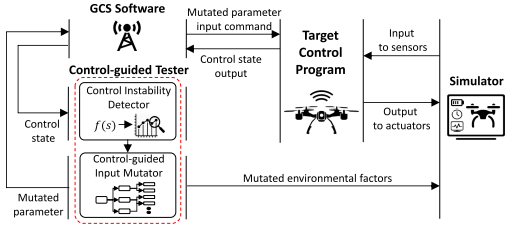
\includegraphics[width=\linewidth]{rvfuzzer.png} %
    \caption{rvfuzzer's arch.}	
    \label{fig:rvfuzzer}
\end{figure}
\subsection{Results/Evaluation}
In their evaluation of RVFUZZER on two popular RV control programs (ArduPilot [15] and PX4 [24]), a total of 89 input validation bugs are found, with 87 of them being zero-day bugs.
\subsection{Limitations/Comments}
The control parameters may have dependencies on one another.  In this work, they consider the subject control program binary as a black box and take a pragmatic approach by only revealing part of such inter-dependencies. A more generic approach to control parameter dependency derivation – possibly based on source code and a formal control model – is left as future work.

There has been no standard safety testing framework created for RVs. We believe that RVFUZZER’s post-production, black-box-based vetting will serve as a useful complement to standardized safety testing during RV design and production.

\newpage
\section{ProFuzzer: On-the-fly Input Type Probing for Better
Zero-day Vulnerability Discovery @S\&P'19}
\subsection{Background/Problems}
Existing mutation based fuzzers tend to randomly mutate the input of a program without understanding its underlying syntax and semantics.  This information (fields and their semantics) may not be documented and available to the fuzzer, and can be hard to recover without going through an in-depth heavyweight analysis procedure. 
\subsection{Methods/Techniques}
 In this paper, the authors propose a novel on-the-fly probing technique (called ProFuzzer, Fig.\ref{fig:profuzzer}) that automatically recovers and understands input fields of critical importance to vulnerability discovery during a fuzzing process and intelligently adapts the mutation strategy to enhance the chance of hitting zero-day targets. Since such probing is transparently piggybacked to the regular fuzzing, no prior knowledge of the input specification is needed. During fuzzing, individual bytes are first mutated and their fuzzing results are automatically analyzed to link those related together and identify the type for the field connecting them; these bytes are further mutated together following type-specific strategies, which substantially prunes the search space.  They define the probe types generally across all applications, thereby making their technique application agnostic.

ProFuzzer is inspired by two important observations. First, a comprehensive, application-specific and semantically rich input specification is not necessary for fuzzing.  Second, inputs can be understood and their fields and data types can be discovered by directly observing the fuzzing process, particularly the ways the input content is mutated and the program’s execution path variations in response to the mutations. 

\begin{figure}[h]
    \centering
    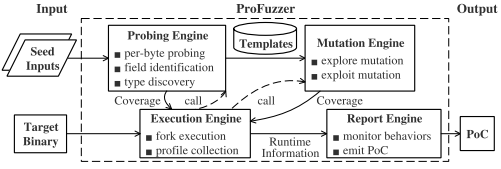
\includegraphics[width=\linewidth]{profuzzer.png} %
    \caption{profuzzer's arch.}	
    \label{fig:profuzzer}
\end{figure}
\subsection{Results/Evaluation}
Eexperiments on standard benchmarks and real-world applications show that ProFuzzer substantially outperforms AFL and its optimized version AFLFast, as well as other state-of-art fuzzers including VUzzer, Driller and QSYM. Within two months, it exposed 42 zero-days in 10 intensively tested programs, generating 30 CVEs.
\subsection{Limitations/Comments}
Currently, the exploitation mutation procedure requires domain knowledge and manual efforts.  A future work is the automatic learning of exploitation rules from a larger pool of PoC.

Review the assumptions that the target application has the following properties. First, its execution is deterministic: that is, given the same input, multiple executions of the application all follow the same execution path and yield the same result. Second, initial valid seed inputs of reasonable size are available. Third, if the validation on certain bytes fails, the execution will quickly terminate, which means that an exceptional execution has a shorter execution path than a normal one. 
\newpage
\section{RetroWrite: Statically Instrumenting COTS Binaries for Fuzzing and Sanitization @S\&P'20}
\subsection{Background/Problems}
The current state of the art for applying fuzzing or sanitization to binaries is dynamic binary translation, which has prohibitive performance overhead. The alternate technique, static binary rewriting, cannot fully recover symbolization information and hence has difficulty modifying binaries to track code coverage for fuzzing or to add security checks for sanitizers.
\subsection{Methods/Techniques}
In this paper, the authors show that static binary rewriting, leveraging reassembleable assembly, can produce sound and efficient code for an important class of binaries: \emph{64-bit position-independent code (PIC)}. Notably, such binaries include third party shared libraries, the analysis of which is the most pressing use-case for such a rewriter. The rewriting technique, called RetroWrite (Fig.\ref{fig:retrowrite}), leverages relocation information which is required for position independent code, and produces assembly files that can be reassembled into binaries. 
\begin{figure}[h]
    \centering
    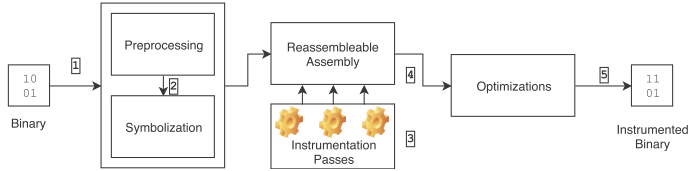
\includegraphics[width=\linewidth]{retrowrite.png} %
    \caption{retrowrite's arch.}	
    \label{fig:retrowrite}
\end{figure}
\subsection{Results/Evaluation}
Binaries rewritten for coverage-guided fuzzing using RetroWrite are identical in performance to compiler-instrumented binaries and outperform the default QEMU-based instrumentation by 4.5x while triggering more bugs. Their implementation of binary-only Address Sanitizer is 3x faster than Valgrind’s memcheck, the state-of-the-art binary-only memory checker, and detects 80\% more bugs in the evaluation.  Available at: \url{https://github.com/HexHive/retrowrite}.
\subsection{Limitations/Comments}
a) Support for C++ Binaries: The current implementation of RetroWrite cannot rewrite C++ binaries safely due to missing symbolization for C++ exception handlers. 

b) Closing the Performance Gap:  Another opportunity to reduce overhead is to remove unnecessary checks when a memory access is known to be safe, e.g., accessing variables on stack through constant offsets from the stack top. 

c) Limitations of ASan-retrowrite: The limitations of ASan-retrowrite on stack and global sections are fundamental to static binary rewriting. To improve precision on stack and data sections, we may need to trade-off soundness or scalability. One attractive option is to use local symbolic execution to track base-pointers and disambiguate references.  

d) Obfuscation: To protect intellectual property, some vendors ship obfuscated binaries. Retrowrite does not address obfuscation. Binary unpacking is usually specific to the obfuscation scheme used; and an obfuscated binary may be rewritten by RetroWrite, after it is pre-processed by a de-obfuscation step [57], [58].
\newpage
\end{document}
